\documentclass{standalone}
\usepackage{tikz}
\usetikzlibrary{patterns, positioning}


\begin{document}
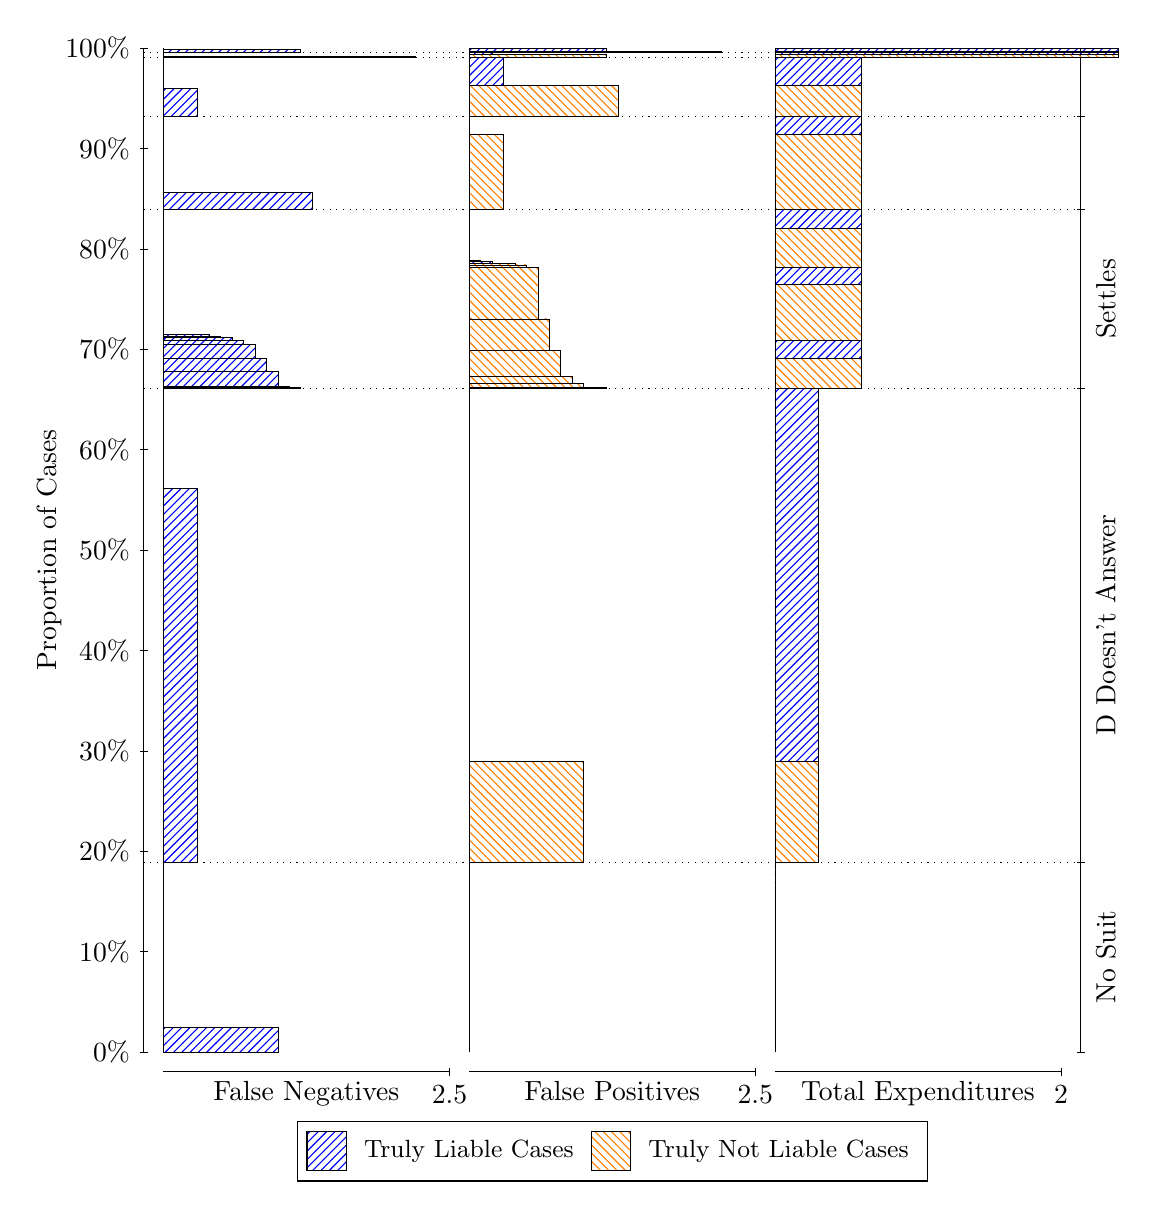
\begin{tikzpicture}
\draw[black, very thin] (1.5,1.75) -- (1.5,14.5);
\node[rotate=90, text=black, anchor=center] at (0.3, 8.125) {Proportion of Cases};
\draw[black, very thin] (1.45,1.75) -- (1.55,1.75);
\node[text=black, anchor=east] at (1.45, 1.75) {0\%};
\draw[black, very thin] (1.45,3.025) -- (1.55,3.025);
\node[text=black, anchor=east] at (1.45, 3.025) {10\%};
\draw[black, very thin] (1.45,4.3) -- (1.55,4.3);
\node[text=black, anchor=east] at (1.45, 4.3) {20\%};
\draw[black, very thin] (1.45,5.575) -- (1.55,5.575);
\node[text=black, anchor=east] at (1.45, 5.575) {30\%};
\draw[black, very thin] (1.45,6.85) -- (1.55,6.85);
\node[text=black, anchor=east] at (1.45, 6.85) {40\%};
\draw[black, very thin] (1.45,8.125) -- (1.55,8.125);
\node[text=black, anchor=east] at (1.45, 8.125) {50\%};
\draw[black, very thin] (1.45,9.4) -- (1.55,9.4);
\node[text=black, anchor=east] at (1.45, 9.4) {60\%};
\draw[black, very thin] (1.45,10.675) -- (1.55,10.675);
\node[text=black, anchor=east] at (1.45, 10.675) {70\%};
\draw[black, very thin] (1.45,11.95) -- (1.55,11.95);
\node[text=black, anchor=east] at (1.45, 11.95) {80\%};
\draw[black, very thin] (1.45,13.225) -- (1.55,13.225);
\node[text=black, anchor=east] at (1.45, 13.225) {90\%};
\draw[black, very thin] (1.45,14.5) -- (1.55,14.5);
\node[text=black, anchor=east] at (1.45, 14.5) {100\%};

\draw[black, very thin] (13.4,1.75) -- (13.4,14.5);
\draw[black, very thin] (13.35,1.75) -- (13.45,1.75);
\node[anchor=west] at (13.35, 1.75) {};
\draw[black, very thin] (13.35,4.1619) -- (13.45,4.1619);
\node[anchor=west] at (13.35, 4.1619) {};
\draw[black, very thin] (13.35,10.181) -- (13.45,10.181);
\node[anchor=west] at (13.35, 10.181) {};
\draw[black, very thin] (13.35,12.447) -- (13.45,12.447);
\node[anchor=west] at (13.35, 12.447) {};
\draw[black, very thin] (13.35,13.628) -- (13.45,13.628);
\node[anchor=west] at (13.35, 13.628) {};
\draw[black, very thin] (13.35,14.378) -- (13.45,14.378);
\node[anchor=west] at (13.35, 14.378) {};
\draw[black, very thin] (13.35,14.44) -- (13.45,14.44);
\node[anchor=west] at (13.35, 14.44) {};
\draw[black, very thin] (13.35,14.5) -- (13.45,14.5);
\node[anchor=west] at (13.35, 14.5) {};

\draw[black, very thin, pattern color=blue, pattern=north east lines] (1.75,1.75) rectangle (3.2033,2.0669);
\draw[black, very thin, pattern color=orange, pattern=north west lines] (1.75,2.0669) rectangle (1.75,4.1619);
\draw[black, very thin, pattern color=blue, pattern=north east lines] (1.75,4.1619) rectangle (2.186,8.9051);
\draw[black, very thin, pattern color=orange, pattern=north west lines] (1.75,8.9051) rectangle (1.75,10.181);
\draw[black, very thin, pattern color=blue, pattern=north east lines] (1.75,10.181) rectangle (3.494,10.186);
\draw[black, very thin, pattern color=blue, pattern=north east lines] (1.75,10.186) rectangle (3.3487,10.2);
\draw[black, very thin, pattern color=blue, pattern=north east lines] (1.75,10.2) rectangle (3.2033,10.39);
\draw[black, very thin, pattern color=blue, pattern=north east lines] (1.75,10.39) rectangle (3.058,10.393);
\draw[black, very thin, pattern color=blue, pattern=north east lines] (1.75,10.393) rectangle (3.058,10.56);
\draw[black, very thin, pattern color=blue, pattern=north east lines] (1.75,10.56) rectangle (2.9127,10.738);
\draw[black, very thin, pattern color=blue, pattern=north east lines] (1.75,10.738) rectangle (2.7673,10.789);
\draw[black, very thin, pattern color=blue, pattern=north east lines] (1.75,10.789) rectangle (2.622,10.827);
\draw[black, very thin, pattern color=blue, pattern=north east lines] (1.75,10.827) rectangle (2.4767,10.84);
\draw[black, very thin, pattern color=blue, pattern=north east lines] (1.75,10.84) rectangle (2.3313,10.86);
\draw[black, very thin, pattern color=orange, pattern=north west lines] (1.75,10.86) rectangle (1.75,12.447);
\draw[black, very thin, pattern color=blue, pattern=north east lines] (1.75,12.447) rectangle (3.6393,12.667);
\draw[black, very thin, pattern color=orange, pattern=north west lines] (1.75,12.667) rectangle (1.75,13.628);
\draw[black, very thin, pattern color=blue, pattern=north east lines] (1.75,13.628) rectangle (2.186,13.983);
\draw[black, very thin, pattern color=orange, pattern=north west lines] (1.75,13.983) rectangle (1.75,14.378);
\draw[black, very thin, pattern color=blue, pattern=north east lines] (1.75,14.378) rectangle (4.9473,14.394);
\draw[black, very thin, pattern color=orange, pattern=north west lines] (1.75,14.394) rectangle (1.75,14.44);
\draw[black, very thin, pattern color=blue, pattern=north east lines] (1.75,14.44) rectangle (3.494,14.484);
\draw[black, very thin, pattern color=orange, pattern=north west lines] (1.75,14.484) rectangle (1.75,14.5);
\draw[black, very thin, pattern color=orange, pattern=north west lines] (5.6333,1.75) rectangle (5.6333,3.845);
\draw[black, very thin, pattern color=blue, pattern=north east lines] (5.6333,3.845) rectangle (5.6333,4.1619);
\draw[black, very thin, pattern color=orange, pattern=north west lines] (5.6333,4.1619) rectangle (7.0867,5.4374);
\draw[black, very thin, pattern color=blue, pattern=north east lines] (5.6333,5.4374) rectangle (5.6333,10.181);
\draw[black, very thin, pattern color=orange, pattern=north west lines] (5.6333,10.181) rectangle (7.3773,10.188);
\draw[black, very thin, pattern color=orange, pattern=north west lines] (5.6333,10.188) rectangle (7.232,10.194);
\draw[black, very thin, pattern color=orange, pattern=north west lines] (5.6333,10.194) rectangle (7.0867,10.238);
\draw[black, very thin, pattern color=orange, pattern=north west lines] (5.6333,10.238) rectangle (6.9413,10.328);
\draw[black, very thin, pattern color=orange, pattern=north west lines] (5.6333,10.328) rectangle (6.796,10.656);
\draw[black, very thin, pattern color=orange, pattern=north west lines] (5.6333,10.656) rectangle (6.6507,11.059);
\draw[black, very thin, pattern color=orange, pattern=north west lines] (5.6333,11.059) rectangle (6.5053,11.717);
\draw[black, very thin, pattern color=orange, pattern=north west lines] (5.6333,11.717) rectangle (6.36,11.747);
\draw[black, very thin, pattern color=orange, pattern=north west lines] (5.6333,11.747) rectangle (6.2147,11.768);
\draw[black, very thin, pattern color=blue, pattern=north east lines] (5.6333,11.768) rectangle (5.924,11.788);
\draw[black, very thin, pattern color=blue, pattern=north east lines] (5.6333,11.788) rectangle (5.7787,11.801);
\draw[black, very thin, pattern color=blue, pattern=north east lines] (5.6333,11.801) rectangle (5.6333,12.447);
\draw[black, very thin, pattern color=orange, pattern=north west lines] (5.6333,12.447) rectangle (6.0693,13.408);
\draw[black, very thin, pattern color=blue, pattern=north east lines] (5.6333,13.408) rectangle (5.6333,13.628);
\draw[black, very thin, pattern color=orange, pattern=north west lines] (5.6333,13.628) rectangle (7.5227,14.023);
\draw[black, very thin, pattern color=blue, pattern=north east lines] (5.6333,14.023) rectangle (6.0693,14.378);
\draw[black, very thin, pattern color=orange, pattern=north west lines] (5.6333,14.378) rectangle (7.3773,14.424);
\draw[black, very thin, pattern color=blue, pattern=north east lines] (5.6333,14.424) rectangle (5.924,14.44);
\draw[black, very thin, pattern color=orange, pattern=north west lines] (5.6333,14.44) rectangle (8.8307,14.456);
\draw[black, very thin, pattern color=blue, pattern=north east lines] (5.6333,14.456) rectangle (7.3773,14.5);
\draw[black, very thin, pattern color=orange, pattern=north west lines] (9.5167,1.75) rectangle (9.5167,3.845);
\draw[black, very thin, pattern color=blue, pattern=north east lines] (9.5167,3.845) rectangle (9.5167,4.1619);
\draw[black, very thin, pattern color=orange, pattern=north west lines] (9.5167,4.1619) rectangle (10.062,5.4374);
\draw[black, very thin, pattern color=blue, pattern=north east lines] (9.5167,5.4374) rectangle (10.062,10.181);
\draw[black, very thin, pattern color=orange, pattern=north west lines] (9.5167,10.181) rectangle (10.607,10.559);
\draw[black, very thin, pattern color=blue, pattern=north east lines] (9.5167,10.559) rectangle (10.607,10.788);
\draw[black, very thin, pattern color=orange, pattern=north west lines] (9.5167,10.788) rectangle (10.607,11.499);
\draw[black, very thin, pattern color=blue, pattern=north east lines] (9.5167,11.499) rectangle (10.607,11.712);
\draw[black, very thin, pattern color=orange, pattern=north west lines] (9.5167,11.712) rectangle (10.607,12.209);
\draw[black, very thin, pattern color=blue, pattern=north east lines] (9.5167,12.209) rectangle (10.607,12.447);
\draw[black, very thin, pattern color=orange, pattern=north west lines] (9.5167,12.447) rectangle (10.607,13.408);
\draw[black, very thin, pattern color=blue, pattern=north east lines] (9.5167,13.408) rectangle (10.607,13.628);
\draw[black, very thin, pattern color=orange, pattern=north west lines] (9.5167,13.628) rectangle (10.607,14.023);
\draw[black, very thin, pattern color=blue, pattern=north east lines] (9.5167,14.023) rectangle (10.607,14.378);
\draw[black, very thin, pattern color=orange, pattern=north west lines] (9.5167,14.378) rectangle (13.877,14.424);
\draw[black, very thin, pattern color=blue, pattern=north east lines] (9.5167,14.424) rectangle (13.877,14.44);
\draw[black, very thin, pattern color=orange, pattern=north west lines] (9.5167,14.44) rectangle (13.877,14.456);
\draw[black, very thin, pattern color=blue, pattern=north east lines] (9.5167,14.456) rectangle (13.877,14.5);
\draw[black, dotted] (1.5,4.1619) -- (13.4,4.1619);
\draw[black, dotted] (1.5,10.181) -- (13.4,10.181);
\draw[black, dotted] (1.5,12.447) -- (13.4,12.447);
\draw[black, dotted] (1.5,13.628) -- (13.4,13.628);
\draw[black, dotted] (1.5,14.378) -- (13.4,14.378);
\draw[black, dotted] (1.5,14.44) -- (13.4,14.44);
\draw[black, very thin] (1.75,1.5) -- (5.3833,1.5);
\node[text=black, anchor=north] at (3.5667, 1.5) {False Negatives};
\draw[black, very thin] (5.3833,1.45) -- (5.3833,1.55);
\node[text=black, anchor=north] at (5.3833, 1.45) {2.5};

\draw[black, very thin] (5.6333,1.5) -- (9.2667,1.5);
\node[text=black, anchor=north] at (7.45, 1.5) {False Positives};
\draw[black, very thin] (9.2667,1.45) -- (9.2667,1.55);
\node[text=black, anchor=north] at (9.2667, 1.45) {2.5};

\draw[black, very thin] (9.5167,1.5) -- (13.15,1.5);
\node[text=black, anchor=north] at (11.333, 1.5) {Total Expenditures};
\draw[black, very thin] (13.15,1.45) -- (13.15,1.55);
\node[text=black, anchor=north] at (13.15, 1.45) {2};

\node[text=black, centered, rotate=90] at (13.72, 2.9559) {No Suit};
\node[text=black, centered, rotate=90] at (13.72, 7.1713) {D Doesn't Answer};
\node[text=black, centered, rotate=90] at (13.72, 11.314) {Settles};





\draw (7.449999999999999,1.5) node[draw=none] (baseCoordinate) {};
\begin{scope}[align=center]
        \matrix[scale=0.5, draw=black, below=0.5cm of baseCoordinate, nodes={draw}, column sep=0.1cm]{
            \node[rectangle, draw, minimum width=0.5cm, minimum height=0.5cm, pattern color=blue, pattern=north east lines] {}; &
            \node[draw=none, font=\small, text=black] (B) {Truly Liable Cases}; &
            \node[rectangle, draw, minimum width=0.5cm, minimum height=0.5cm, pattern color=orange, pattern=north west lines] {}; &
            \node[draw=none, font=\small, text=black] (B) {Truly Not Liable Cases}; \\
            };
\end{scope}

\end{tikzpicture}
\end{document}